\chapter{Preliminary Quantum Mechanics} \label{chp:quantum}
\epigraph{I do not like it, and I am sorry I ever had anything to do with it.}{Erwin Schrödinger, \cite{noauthor_quantum_2005}}
\begin{figure}[H]
	\centering
	\captionsetup[subfigure]{labelformat=empty}
	\tikzsetnextfilename{quantum_entanglement}
	\copyrightbox[l]{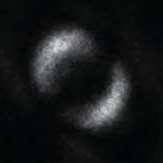
\includegraphics[scale=1]{../Images/entanglement.jpeg}}{Science Advances, Vol. 5, no.7 (2019)}
	\caption{The first ever image of quantum entanglement, where two groups of particles are sharing the physical state $\Psi(\bs{x})$, was published by \citet{moreau_imaging_2019} with the title \textit{Imaging Bell-type nonlocal behavior} in 2019.}
	\label{fig:entanglement}
\end{figure}

The quantum theory is a fundamental theory that describes nature at the smallest scales, typically used to explain the behavior of atoms and subatomic particles. Although the theory in principle holds for systems containing a large number of particles as well, the calculations become both comprehensive and expensive as the system size increases, and exact computations are therefore reserved small systems. For larger systems, we in practice need to rely on approximative estimates of the observable, which also fast becomes infeasible when the system size increase.

In the most general form, the theory is based on the time-dependent Schrödinger equation,
\begin{empheq}[box={\mybluebox[5pt]}]{equation}
i\hbar\frac{\partial}{\partial t}\ket{\Psi(\bs{x},t)}=\hat{\mathcal{H}}\ket{\Psi(\bs{x},t)}
\end{empheq}
which describes the state, or the wave function, $\Psi(\bs{x},t)$, of a system with Hamilton operator $\hat{\mathcal{H}}$, known as the Hamiltonian. $\bs{x}=(\bs{r},\sigma)$ specifies the coordinates and the spin of a particle, $\hbar$ is the reduced Planck's constant and $i$ is the solution of the equation $x^2=-1$. As we later will see, the quantum mechanical system is completely specified by the wave function, so by solving the equation we will in principle know anything about the system. 

\citet{schrodinger_undulatory_1926} introduced the now-called Schrödinger equation in a 1926 paper as one of many contributions to the quantum mechanics at that time. Other contributors include \citet{born_zur_1926} who suggested now-standard interpretation of the probability density function as $|\Psi(\bs{x},t)|^2$ in 1926 and his companion \citet{heisenberg_uber_1925}, who formulated the matrix mechanics representation in 1925. However, many physicists were skeptical about the new theory, including Albert Einstein and Schrödinger himself. The theory differed from the classical mechanics in the sense that it was based on a statistical interpretation, with some strange consequences. For instance, the theory allowed negative kinetic energies to occur with the consequence that a particle could \textit{go through} a potential wall, known as quantum tunneling. Later, Einstein \cite{einstein_can_1935} also pointed out that when pairs or groups of particles are generated in ways such that the wave function of each particle cannot be described independently of the other state, they will be affected by each other even at large distances. He called this \textit{"spooky action at a distance"}, and used the observation to argument that the quantum theory had to be incorrect. However, the observation was later proven to be correct and as late as in 2019 the first image of quantum entanglement, as the phenomenon is called, was captured by \citet{moreau_imaging_2019}. This image is presented in figure \eqref{fig:entanglement}.

Today, there is wide agreement in the physics society on the quantum theory. Actually, the theory is the most precisely tested in the history of science, where computed observable of atoms agree perfectly with experiments. Most notably, quantum electrodynamical calculations of the fine structure constant $\alpha$ are, by \citet{odom_new_2006}, found to agree with experiments within ten parts in a billion, $10^{-8}$.\bigskip

In this chapter, we will first state the postulates of quantum mechanics, and thereafter we discuss the time-independent Schrödinger equation and challenges related to solving it. As we will see, every observable in quantum mechanics is associated with an operator. The consequence is that all obtained values are identified with standard errors which are also important to specify in order to present the accuracy of the value. In that manner, quantum mechanics is based on statistics, and in section \ref{sec:statisticalinterpretation} we discuss the statistical interpretation of the theory. The variational principle states that the ground state energy is the lowest possible energy calculated, so by minimizing the energy in a variational scheme, a ground state energy estimation can be obtained. Other things discussed are the quantum numbers, which are the values that give acceptable solutions to the Schrödinger equation, and the virial theorem, which relates kinetic and potential energy. 

Albeit the quantum mechanics will make up the framework for this work, we will in this chapter only discuss the theory needed for the work, and this is therefore not meant as an encyclopedia to quantum mechanics. For a complete introduction to the topic, \textit{Introduction to Quantum Mechanics} written by \citet{griffiths_introduction_2005} serves as an excellent read. Before we get started, we make a few assumptions in order to simplify our problem. The most important ones are specified below with an explanation of why they are valid.

\begin{itemize}
	\item \textbf{Point-like particles:} First, all particles involved will be assumed to be point-like, i.e., they lack spatial extension. For electrons, this makes sense since they, as far as we know, do not extend. The assumption is also applied to the nucleus in atomic systems, but it still makes sense since the distance from the nucleus to the electrons is known to be much larger than the nucleus extension.
	
	\item \textbf{Non-relativistic spacetime:}  Second, we operate in the non-relativistic spacetime, which is an excellent approximation as long as we do not approach the speed of light and we do not involve strong forces. Applying classical physics, we can find that the speed of the electron in a hydrogen atom is about 1\% of the speed of light. Even though the electrons achieve higher velocities in heavy atoms, we do not need to worry about it as we will stick to the lighter atoms. In the quantum dots, this assumption holds even for large systems, as the velocity and density will still be sufficiently low.
	
	\item For specific systems, we might make new assumptions and approximations. For instance, for atomic systems, we will assume that the nucleus is at rest. Those approximations will be discussed consecutively. 
\end{itemize}

\section{The postulates of quantum mechanics} \label{sec:postulates}
Quantum mechanics is characterized by a set of fundamental axioms that make up the base of the theory. As we assume that they always hold, every statement in quantum mechanics is based on them, and it is, therefore, natural to list them now in the beginning. They can be formulated by six postulates, in the following way:

\begin{enumerate}
	\item \textit{"The state of a quantum mechanical system is completely specified by the wave function $\Psi(\bs{x},t)$."}
	
	\item \textit{"To every observable in classical mechanics, there corresponds a linear, Hermitian operator in quantum mechanics."}
	
	\item \textit{"In any measurement of the observable associated with an operator $\hat{O}$, the only values that will ever be observed are the eigenvalues $o$ which satisfy $\hat{O}\Psi(\bs{x},t)=o\Psi(\bs{x},t)$."}
	
	\item \textit{"The expectation value of the observable corresponding to operator $\hat{O}$ is given by
		$$\langle\hat{O}\rangle=\frac{\int d\bs{x}dt\Psi^*(\bs{x},t)\hat{O}\Psi(\bs{x},t)}{\int d\bs{x}dt\Psi^*(\bs{x},t)\Psi(\bs{x},t)}.\textit{"}$$}
	
	\item \textit{"The wave function evolves in time according to the time-dependent Schrödinger equation,
		$$\hat{\mathcal{H}}\Psi(\bs{x},t)=i\hbar\frac{\partial\Psi(\bs{x},t)}{\partial t}.\textit{"}$$}
	
	\item \textit{"The total wave function must be anti-symmetric concerning the interchange of all coordinates of one fermion with those of another. Electronic spin must be included in this set of coordinates."} 
\end{enumerate}
All the postulates will be used in this work, and they will be described in detail when we need them. Even though we will look at stationary states only, even the time-dependent Schrödinger from the fifth postulate will be discussed due to the description of the diffusion Monte Carlo method in section \ref{sec:dmc}. The other will be covered in the current and the next chapter. The formulation of the presented postulates are taken from Ref. \cite{sherrill_david_postulates_2003}.

\section{The Schrödinger equation} \label{sec:schrodinger}
We have already presented the time-dependent Schrödinger equation on several occasions, but as mentioned above, we will in this work study stationary systems only. If we also recall that the particles are assumed to be non-relativistic, the focus will be on solving the time-independent non-relativistic Schrödinger equation. By defining $\Psi_n(\bs{x})$ as the wave function of a state $n$ with energy $E_n$, the equation can be expressed as
\begin{empheq}[box={\mybluebox[5pt]}]{equation}
\label{eq:Energy}
\hat{\mathcal{H}}\psin=E_n\psin,
\end{empheq}
where $\hat{\mathcal{H}}$ is the aforementioned Hamiltonian, the total energy operator. By analogy with the classical mechanics, the total mechanical energy is the kinetic and potential energy summarized,
\begin{equation}
\hat{H}=\hat{T}+\hat{V}
\end{equation}
with $\hat{T}$ and $\hat{V}$ as the kinetic and potential energy operators respectively. 

Again from classical mechanics, the kinetic energy of a moving particle of mass $m$ yields $T=p^2/2m$ where $p$ is the (linear) momentum, such that the kinetic energy operator can be represented as 
\begin{equation}
\hat{T}=\frac{\hat{p}^2}{2m},
\end{equation}
according to Ehrenfest's theorem. Further, the momentum operator is $\hat{p}=-i\hbar\hat{\nabla}$ with $\hat{\nabla}$ as the differential operator and the factor $i\hbar$ arising from the canonical commutator relation between the position operator and the momentum operator,
\begin{equation}
[\hat{x},\hat{p}]=\hat{x}\hat{p}-\hat{p}\hat{x}=i\hbar,
\end{equation}
which indicates that the momentum and the position do not \textit{commute}. In other words, the order of the operators in an equation is not arbitrary. The potential, on the other hand, is obviously dependent on the system we want to study. For atomic systems, the potential as a function of the distance from the nucleus can be found from Coulomb's law and reads 
\begin{equation}
V(r)=\frac{1}{4\pi\epsilon_0}\frac{Ze^2}{r},
\label{eq:atompotential}
\end{equation}
where the nucleus is assumed to be at rest at the origin, $k_e=1/4\pi\epsilon_0$ is the Coulomb constant, $Z$ is the atomic number of the nucleus, and $e$ is the elementary charge. For a general potential, the Hamiltonian can be expressed as 
\begin{equation}
\hat{\mathcal{H}}=-\frac{\hbar^2}{2m}\nabla^2+V(r),
\label{eq:oneparticlehamiltonian}
\end{equation}
which is the farthest we can go without specifying the external potential $V(r)$.

By setting up equation \eqref{eq:Energy} with respect to the energies, we obtain an integral,
\begin{equation}
E_n=\frac{\int d\bs{x}\psinc\hat{\mathcal{H}}\psin}{\int d\bs{x}\psinc\psin},
\label{eq:energyintegral}
\end{equation}
which not necessarily is trivial to solve. For almost\footnote{Exceptions include quantum dots of two electrons in two and three dimensions, where Taut has presented semi-analytical energies for a few oscillator frequencies \cite{taut_two_1993,taut_two_1994}.} all many-electron systems, this becomes analytically infeasible due to a two-body interaction term. This will be covered in chapter \ref{chp:manybody}.

As suggested by Max Born, we get the probability density function if we take the dot product between the complex conjugate wave function and the wave function itself,
\begin{equation}
P(\bs{r})=\psinc\psin=|\psin|^2,
\label{eq:pdf}
\end{equation}
so the denominator in equation \eqref{eq:energyintegral} is basically the integral over all the probabilities. If the wave function is normalized correctly, this should always give 1. As a very brief example, we will below calculate the bounding energy of the hydrogen atom.

\subsection{The hydrogen atom} \label{sec:hydrogen}
We presented the one-particle Hamiltonian in equation \eqref{eq:oneparticlehamiltonian}, and the potential from the nucleus in equation \eqref{eq:atompotential}. By introducing the Bohr radius,
\begin{equation}
a_0=\frac{4\pi\epsilon_0\hbar^2}{m_eZe^2},
\end{equation}
we can set up the total Hamiltonian as
\begin{equation}
\hat{\mathcal{H}}\cdot\frac{(4\pi\epsilon_0)^2\hbar^2}{m_eZ^2e^4}=-\frac{1}{2}a_0^2\nabla^2-\frac{a_0}{r},
\end{equation}
where we have multiplied all the terms by the factor $(4\pi\epsilon_0)^2\hbar^2/m_eZ^2e^4$ in order to make the equation dimensionless. We can further scale the energy as $E\leftarrow E\cdot (4\pi\epsilon_0)^2\hbar^2/m_eZ^2e^4$ and the distance as $r\leftarrow r/a_0$, which both are dimensionless, and obtain the Hamiltonian
\begin{equation}
\hat{\mathcal{H}}=-\frac{1}{2}\nabla^2-\frac{1}{r},
\end{equation}
where all quantities are in Hartree atomic units.

The hydrogen ground state wave function is well-known and reads
\begin{equation}
\Psi(r)=\frac{1}{\sqrt{\pi}}e^{-r}
\end{equation}
in atomic units. The binding energy in Hydrogen is found from the Schrödinger equation in equation \eqref{eq:Energy}, and gives
\begin{equation}
\hat{\mathcal{H}}\Psi(r)=\bigg(-\frac{1}{2}\nabla^2-\frac{1}{r}\bigg)\Psi(r)=-\frac{1}{2}\Psi(r),
\end{equation}
which indicates that $E_0=-0.5$.

\section{Statistical interpretation} \label{sec:statisticalinterpretation}
In equation \eqref{eq:energyintegral}, we found the expectation value of the energy using the Hamiltonian, which is the energy operator. By the second postulate of quantum mechanics, every observable in the classical mechanics is associated with such a Hermitian operator $\hat{O}$ related to an expectation value $\langle \hat{O}\rangle$ in the same way,
\begin{equation}
\langle \hat{O}\rangle=\frac{\int d\bs{r}\psinc\hat{O}\psin}{\int d\bs{r}\psinc\psin}.
\label{eq:generalexp}
\end{equation}
As a consequence, there is always an uncertainty associated with a quantum mechanical calculation, such that we can only tell the probability of measuring something. The uncertainty is usually described by the variance, which for a set of independent measurements is given by
\begin{equation}
\sigma^2=\langle \hat{O}^2\rangle-\langle \hat{O}\rangle^2.
\label{eq:variance}
\end{equation}
If there are correlations between the measurements, this expression underestimates the actual sampling variance as the \textit{covariance} is not taken into account, which is detailed in section \ref{sec:variance}. If we take the square root of the variance, we obtain the standard deviation, which is the quantity given as the standard error in the results. From the standard deviation, a variety of mathematical inequalities follows, where Heisenberg's uncertainty principle is the most famous. It states that the more precisely the position of some particle is determined, the less precisely its momentum can be known, and is mathematically presented as
\begin{empheq}[box={\mybluebox[5pt]}]{equation}
\sigma_x\sigma_p\geq\frac{\hbar}{2},
\end{empheq}
where $\sigma_x$ is the standard deviation of the position and $\sigma_p$ is the standard deviation of the momentum.

The general expected value in equation \eqref{eq:generalexp} is expressed using the Schrödinger wave mechanics picture, but it can also be written in terms of, for instance, the Heisenberg picture applying matrices. However, the standard formalism today in most branches of the quantum mechanics is the Dirac notation, which relates the Schrödinger picture and the Heisenberg picture elegantly. Using this, the expectation value from equation \eqref{eq:generalexp} reads
\begin{equation}
\langle \hat{O}\rangle=\frac{\mel{\Psi}{\hat{O}}{\Psi}}{\braket{\Psi}{\Psi}}
\end{equation}
where $\bra{\Psi}$ is called the \textit{bra} and $\ket{\Psi}$ is called the \textit{ket}. For that reason, the formalism is also called bracket formalism. Usually, the wave function is assumed to be normalized, which further simplifies the expected value to
\begin{equation}
\langle \hat{O}\rangle=\mel{\Psi}{\hat{O}}{\Psi},
\end{equation}
and will henceforth be assumed. More information about the Dirac formalism can be found in Appendix \ref{app:dirac}. 

\section{The variational principle} \label{sec:variationalprinciple}
In the equations above, the presented wave functions are assumed to be the exact eigenfunctions of the Hamiltonian. However, often we do not know the exact wave functions, and we need to guess what the wave functions might be. In those cases, we apply the variational principle, which states that only the exact ground state wave function can give the ground state energy. All other wave functions that fulfill the required properties (see section \ref{sec:wavefunction}) give higher energies, and mathematically we can express the statement as
\begin{empheq}[box={\mybluebox[5pt]}]{equation}
E_0\leq\mel{\Psi}{\hat{\mathcal{H}}}{\Psi},
\label{eq:variationalprinciple}
\end{empheq}
where $\Psi$ is an arbitrary wave function. The variational method is a way of estimating the energy ground state, which is based on the variational principle. Most notably, the variational Monte Carlo method is named after the principle and attempts to solve the integrals directly by varying a trial wave function. The variational principle ensures that the obtained energy never goes below the ground state energy, as further described in chapter \ref{chp:methods}. Other methods that apply the variational method are the famous Hartree-Fock method and the infamous coupled cluster method.

\section{Quantum numbers}
Unlike in classical mechanics, all the observable in quantum mechanics are discrete or \textit{quantized}, which means that the $n$ associated with $E_n$ above cannot take any number. $n$ can only take positive integers and is named the principal quantum number. We also have other quantum numbers identified with the angular momentum and spin as described below.

\subsection*{Principal}
The \textbf{principal} quantum number describes the electron shell, and can take all positive integers, $n\in[1,2,3,\hdots)$. As $n$ increases, the electron excites to a higher shell such that also the energy increases. In general, $E_1<E_2<E_3\hdots$ as long as all other quantum numbers are fixed. The electron shells can again be split up in subshells, requiring more quantum numbers.

\subsection*{Angular}
An electron shell can possibly have more than one subshell, described by the \textbf{angular} quantum number $l$. $l$ can take all non-negative integers up to $n$, $l\in[0,1,\hdots n-1]$, such that the degeneracy of subshells in a shell is simply $n$. In atoms, the angular quantum number describes the shape of the shell, where $l=0$ gives a spherical shape, $l=1$ gives a polar shape while $l=2$ gives a cloverleaf shape. 

\subsection*{Magnetic}
We also have a \textbf{magnetic} quantum number, $m_l$, which has the range $-l,-l+1,\hdots,l-1,l$. If $l$ describes the shape of a shell, $m_l$ specifies its orientation in space. This quantum number was first observed under the presence of a magnetic field, hence the name.

\subsection*{Spin}
The \textbf{spin} quantum number, $s$, gives the spin of a particle, which can just be seen as a particle's property. Particles are often classified into two groups depending on the spin because of their different behavior: \textbf{bosons} have integer spin, while \textbf{fermions} have half-integer spin. Electrons and protons have spin $s=1/2$, which makes them fermions.

\subsection*{Spin projection}
The last number we will discuss is the \textbf{spin projection} quantum number $m_s$. It has the range $-s,-s+1,\hdots,s-1,s$, and is therefore related to the spin quantum number in the same way as the magnetic number $m_l$ is related to the angular number $l$. Electrons can for that reason take the values $m_s=+1/2$ or $m_s=-1/2$, such that there are two groups of electrons. The consequences will be discussed in the section \ref{sec:wavefunction}.

\section{The virial theorem} \label{sec:virial}
The virial theorem relates the kinetic energy to the potential energy, and makes it possible to find the (time) average of the kinetic energy even for complex systems. The classical statement of the theorem was formulated during the 19th century and named by \citet{clausius_xvi._1870} in 1870. It is in the most general form given by 
\begin{empheq}[box={\mybluebox[5pt]}]{equation}
\langle\hat{T}\rangle=-\frac{1}{2}\sum_{i=1}^N\langle\bs{F}_i\cdot\bs{r}_i\rangle_t,
\label{eq:virialtheorem}
\end{empheq}
where $\bs{F}_i$ represents the force on particle $i$ at position $\bs{r}_i$. The quantum mechanical version was proven by \citet{fock_bemerkung_1930} in a 1930 paper, where the expectation value of the force is represented with $d\langle p\rangle/dt$. For potential sources in the form of $V_i=ar^{n_i}$, we can use Ehrenfest's theorem to express the virial theorem in a simpler fashion,
\begin{equation}
2\langle \hat{T} \rangle = \sum_{i}n_i\langle \hat{V}_{i} \rangle.
\label{eq:simplevirial}
\end{equation}
The same expression can be found in classical physics as well, using the relation $\bs{F}=-\nabla V$. The virial theorem requires that the system is in a bound state. An example on a system that does not fulfill the requirements, is a comet that has enough kinetic energy to escape a planet's gravitational field. 

On the other hand, the hydrogen atom, discussed in section \ref{sec:hydrogen}, satisfies the virial theorem as the potential is in the form of $V(r)\propto r^{-1}$ and the electron is bounded. For that particular case, the virial theorem reads $2\langle\hat{T}\rangle=-\langle\hat{V}\rangle$, which means that $\langle\hat{H}\rangle=\langle\hat{V}\rangle/2$. However, if we add another electron and get a hydrogen anion, the simplified virial theorem in equation \eqref{eq:simplevirial} breaks down because of the interaction.

It is also important to emphasize that the expectation value discussed above is, in principle, the time average of the operator. However, if the ergodic hypothesis holds for the system, i.e., the ensemble average is equal to the time average, an ensemble average can also be taken \cite{flyvbjerg_error_1989}.

\iffalse
\subsubsection*{Angular Momentum and Spin}
Relation between the angular and spin quantum number

(One last analogy with the classical mechanics)

If we again go back to the classical mechanics, the angular momentum $\bs{L}_r=\bs{R}\cross\bs{p}$ around an axis at distance $|\bs{R}|$ from the mass center and the angular momentum $\bs{L}_c=I\bs{\omega}$ around its own mass center is a conserved quantity,
\begin{equation}
\bs{L}_{net} = \bs{L}_r+\bs{L}_c.
\end{equation}
Since the net angular momentum $\bs{L}_{new}$ is just a sum over the angular momentum of all points in a continua around the rotational axis given by the definition of $\bs{L}_r$, both of them are actually the same thing.

In quantum mechanics we have again an analogy, where we define a \textbf{spin} $s$ which describes a particles rotation around its own mass center and a \textbf{angular momentum} $l$ which describes a particles rotation around an external rotational axis. Like in classical physics, the total spin $S$ and the total angular momentum $L$ is a conserved quantity,
\begin{equation}
J=L+S,
\end{equation}
but the transition from $L$ to $S$ is rare compared to the transition from $L_c$ to $L_r$. Spin-orbit coupling. Azimuthal. Quantized.
\fi